% 附章专用计数器
%\newcounter{CFsection}[chapter]
%\renewcommand{\theCFsection}{\stepcounter{CFsection} \textbf{F.\arabic{CFsection}}}
%\newcounter{CFsubsection}[section]
%\renewcommand{\theCFsubsection}{\stepcounter{CFsubsection} \textbf{F.\arabic{CFsection}.\arabic{CFsubsection}}}
%\renewcommand{\theequation}{F.\arabic{equation}}


% 附章专用标题格式
%\titleformat{\chapter}{\bfseries\Huge\color{titlepurple}}{附章 \quad}{0pt}{}
%\titleformat{\section}{\Large\color{titlepurpleb}}{\bfseries{\theCFsection}\quad  }{0pt}{}
%\titleformat{\subsection}{\large\color{titlepurplec}}{\bfseries{\theCFsubsection}\quad  }{0pt}{}


\chapter{补充公式及基本化简方法}
\thispagestyle{empty}
\section{三角函数公式}
\subsection{和差化积}
\begin{equation}
	\boxed{\sin \alpha + \sin \beta = 2 \sin \dfrac{\alpha + \beta}{2}  \cos  \dfrac{\alpha - \beta}{2} }
	\vspace*{0.5em}
\end{equation}
\renewcommand{\arraystretch}{1.6}
\begin{tabular}{l}
\proof \quad $\displaystyle \sin \alpha + \sin \beta = \sin  \left( \dfrac{\alpha + \beta}{2} + \dfrac{\alpha - \beta}{2}\right) + \sin \left( \dfrac{\alpha + \beta}{2} - \dfrac{\alpha - \beta}{2} \right)$\\[-1em]
$\displaystyle = \sin  \dfrac{\alpha + \beta}{2} \cos  \dfrac{\alpha - \beta}{2}  + \cos  \dfrac{\alpha + \beta}{2}\sin  \dfrac{\alpha - \beta}{2} + \sin \dfrac{\alpha + \beta}{2}\cos \dfrac{\alpha - \beta}{2} - \cos \dfrac{\alpha + \beta}{2} \sin \dfrac{\alpha - \beta}{2}$\\
$= 2 \sin \dfrac{\alpha + \beta}{2}  \cos  \dfrac{\alpha - \beta}{2} $
\end{tabular}

\vspace*{1.2em}

\begin{equation}
	\boxed{\sin \alpha - \sin \beta = 2 \cos \dfrac{\alpha + \beta}{2}\sin \dfrac{\alpha- \beta}{2}}
	\vspace*{0.5em}
\end{equation}
\begin{tabular}{l}
	\proof \quad $\displaystyle \sin \alpha - \sin \beta = \sin \left( \dfrac{\alpha + \beta }{2} + \dfrac{\alpha - \beta}{2}\right) - \sin \left( \dfrac{\alpha - \beta}{2} - \dfrac{\alpha - \beta}{2} \right)$ \\[-1em]
	$=\sin \dfrac{\alpha + \beta}{2} \cos \dfrac{\alpha - \beta}{2} + \cos \dfrac{\alpha + \beta}{2}\sin \dfrac{\alpha - \beta}{2} - \sin \dfrac{\alpha + \beta}{2}\cos\dfrac{\alpha - \beta}{2} + \cos \dfrac{\alpha + \beta}{2} \sin \dfrac{\alpha - \beta}{2}$\\
	$= 2 \cos \dfrac{\alpha + \beta}{2} \sin \dfrac{\alpha - \beta}{2}$
\end{tabular}

\vspace*{1.2em}

\begin{equation}
	\boxed{\cos \alpha + \cos \beta = 2 \cos \dfrac{\alpha + \beta}{2}\cos \dfrac{\alpha- \beta}{2}}
	\vspace*{0.5em}
\end{equation}
\begin{tabular}{l}
	\proof \quad $\displaystyle \cos \alpha + \cos \beta = \cos \left( \dfrac{\alpha + \beta }{2} + \dfrac{\alpha - \beta}{2}\right) + \cos \left( \dfrac{\alpha - \beta}{2} - \dfrac{\alpha - \beta}{2} \right)$ \\[-1em]
	$=\cos \dfrac{\alpha + \beta}{2} \cos \dfrac{\alpha - \beta}{2} - \sin \dfrac{\alpha + \beta}{2}\sin \dfrac{\alpha - \beta}{2} + \cos \dfrac{\alpha + \beta}{2} \cos\dfrac{\alpha - \beta}{2} - \sin \dfrac{\alpha + \beta}{2} \sin \dfrac{\alpha - \beta}{2}$\\
	$= 2 \cos \dfrac{\alpha + \beta}{2} \cos \dfrac{\alpha - \beta}{2}$
\end{tabular}

\vspace*{2em}

\begin{equation}
	\boxed{\cos \alpha - \cos \beta = - 2 \sin \dfrac{\alpha + \beta}{2}\sin \dfrac{\alpha- \beta}{2}}
	\vspace*{0.5em}
\end{equation}
\begin{tabular}{l}
	\proof \quad $\displaystyle \cos \alpha - \cos \beta = \cos \left( \dfrac{\alpha + \beta }{2} + \dfrac{\alpha - \beta}{2}\right) - \cos \left( \dfrac{\alpha - \beta}{2} - \dfrac{\alpha - \beta}{2} \right)$ \\[-1em]
	$=\cos \dfrac{\alpha + \beta}{2} \cos \dfrac{\alpha - \beta}{2} - \sin \dfrac{\alpha + \beta}{2}\sin \dfrac{\alpha - \beta}{2} - \cos \dfrac{\alpha + \beta}{2} \cos\dfrac{\alpha - \beta}{2} + \sin \dfrac{\alpha + \beta}{2} \sin \dfrac{\alpha - \beta}{2}$\\
	$= - 2 \sin \dfrac{\alpha + \beta}{2} \sin \dfrac{\alpha - \beta}{2}$
\end{tabular}

\begin{equation}
	\boxed{\tan \alpha + \tan \beta = \dfrac{\sin \big(\alpha + \beta \big)}{\cos \alpha \cos \beta} }
	\vspace*{0.5em}
\end{equation}
\quad \proof \quad $\displaystyle \tan \alpha + \tan \beta = \dfrac{\sin \alpha}{\cos \alpha} + \dfrac{\sin \beta}{\cos \beta} = \dfrac{\sin \alpha \cos \beta + \cos \alpha + \sin \beta}{\cos \alpha \cos \beta} = \dfrac{\sin \big( \alpha + \beta)}{\cos \alpha \cos \beta}$


\subsection{积化和差}
\vspace*{-1em}
\begin{align}
	\boxed{\sin \alpha \cos \beta = \dfrac 1 2 \Big[\sin \big( \alpha + \beta \big) + \sin \big( \alpha - \beta \big) \Big]} \\[0.5em]
	\boxed{\sin \alpha \sin \beta = -\dfrac 1 2 \Big[\cos \big(\alpha + \beta \big) - \sin \big( \alpha - \beta \big) \Big]} \\[0.5em]
	\boxed{\cos \alpha \sin \beta = \dfrac 1 2 \Big[\sin \big( \alpha + \beta \big) - \sin \big( \alpha - \beta \big) \Big]} \\[0.5em]
	\boxed{\cos \alpha \cos \beta = \dfrac 1 2 \Big[\cos \big(\alpha + \beta \big) + \cos \big( \alpha - \beta \big) \Big]}
\end{align}

\subsection{降幂公式(升幂公式)}
由二倍角公式,得
\begin{equation*}
	\cos 2 \alpha = \cos^2 \alpha - \sin^2 \alpha = 1 - 2\sin^2 \alpha = 2 \cos^2 \alpha - 1
\end{equation*}

\noindent 从而推导出以下公式
\begin{equation}
	\boxed{\sin^2 \alpha = \dfrac{1 - \cos 2 \alpha }{2}} \qquad \qquad \boxed{\cos^2 \alpha = \dfrac{1 + \cos 2 \alpha }{2}} \qquad \qquad \boxed{\tan^2 \alpha = \dfrac{1 - \cos 2 \alpha }{1 + \cos 2 \alpha}}
	\vspace*{0.5em}
\end{equation}

\subsection{万能公式}
\begin{equation}
	\boxed{\sin 2 \theta = \dfrac{2 \tan \theta}{1 + \tan^2 \theta}} \qquad \qquad \boxed{\cos 2 \theta = \dfrac{1 - \tan^2 \theta}{1 + \tan^2 \theta}} \qquad \qquad \boxed{\tan 2 \theta = \dfrac{2 \tan \theta}{1 - \tan^2 \theta}}
	\vspace*{0.5em}
\end{equation}
\proof 由二倍角公式,得
\vspace*{-1em}
\begin{align*}
	& \sin 2 \theta = 2 \sin \theta \cos \theta = \dfrac{2 \sin \theta \cos \theta }{\sin^2 \theta + \cos^2 \theta} = \dfrac{2 \tan \theta}{1 + \tan^2 \theta}. \\[0.5em]
	&\cos 2 \theta = \cos^2 \theta - \sin^2 \theta = \dfrac{\cos^2 \theta - \sin^2 \theta}{\cos^2 \theta + \sin^2 \theta} = \dfrac{1 - \tan^2 \theta}{1 + \tan^2 \theta}.\\[0.5em]
	&\tan 2 \theta = \tan (\theta + \theta) = \dfrac{2 \tan\theta}{1 - \tan^2 \theta}.
\end{align*}


\subsection{其他公式}
\vspace*{-1em}
\begin{align}
	\dfrac{1 + \sin \theta}{1 - \sin \theta} = \dfrac{\big(1 + \sin \theta \big)^2}{1 - \sin^2 \theta} = \left( \dfrac{1 + \sin \theta}{\cos \theta} \right)^2 = \big(\csc \theta + \tan \theta \big)^2 \\[0.5em]
	\dfrac{1 + \cos \theta}{1 - \cos \theta} = \dfrac{\big( 1 + \cos \theta \big)^2}{1 - \cos^2 \theta} = \left( \dfrac{1 + \cos \theta}{\sin \theta} \right)^2 = \big( \sec \theta + \cot \theta \big)^2
\end{align}

\subsection{双曲函数公式}
双曲函数有着特别的性质(与三角函数类似)。具体如下:【注:以下性质用双曲函数的定义可以直接证明,故证明省略】
\begin{align}
	\boxed{\ch^2 x - \sh^2 x = 1} \qquad \quad\\[0.5em]
	\boxed{\sh (x + y) = \sh x \,\ch y + \ch x \,\sh y} \\[0.5em]
	\boxed{\sh (x - y) = \sh x \,\ch y - \ch x \,\sh y} \\[0.5em]
	\boxed{\ch (x + y) = \ch x \,\ch y + \sh x \,\sh y} \\[0.5em]
	\boxed{\ch (x - y) = \ch x \,\ch y - \sh x \,\sh y}  
\end{align}

\section{反三角函数公式}
\subsection{反三角函数的运算法则(仅考虑一个周期)}
\vspace*{-1em}
\begin{equation}
	\boxed{\cos \big( \arcsin x \big) = \sin \big( \arccos x \big) = \sqrt{1 - x^2}}
\end{equation}
\proof 设$t = \arcsin x$,则$x = \sin t$,那么\\[-2.2em]
$$
\cos \big(\arcsin x \big) = \cos t = \sqrt{1 - \sin^2 t} = \sqrt{1 - x^2}
\vspace*{-0.5em}
$$
类似可证,
$$
\sin \big( \arccos x \big) = \sqrt{1 - x^2}
$$

\begin{equation}
	\boxed{\arcsin (-x) = - \arcsin x}
\end{equation}
\proof 设$t = \arcsin x$,则$x = \sin t$,那么\\[-2.2em]
$$
\arcsin(-x) = \arcsin(- \sin t) = \arcsin \big[ \sin (-t) \big] = -t = - \arcsin x
\vspace*{-0.5em}
$$

\begin{equation}
	\boxed{\arccos(-x) = \pi - \arccos x}
\end{equation}
\proof 设$t = \arccos x$,则$x = \tan t$,那么\\[-2.2em]
$$
\arctan (-x) = \arctan(- \tan t) = \arctan \big[ \tan (-t) \big] = - t = - \arctan x
\vspace*{-0.5em}
$$

\begin{equation}
	\boxed{ \arccot (-x) = \pi - \arccot x}
\end{equation}
\proof 设$t = \arccot x$,则$x = \cot t$,那么\\[-2.2em]
$$
\arccot (-x) = \arccot(- \cot t) = \arccot (- \cot t) = \arccot \big[ \cot(\pi - t) \big] = \pi - t = \pi - \arccot x
\vspace*{-0.5em}
$$

\begin{equation}
	\boxed{\arcsin x + \arccos x = \arctan x + \arccot x = \dfrac{\pi}{2}}
\end{equation}
\proof 设$t = \arcsin x$,则$x = \sin t$,那么\\[-2.2em]
$$
\arcsin x + \arccos x = t + \arccos(\sin t) = t + \arccos \left[ \cos \left( \dfrac{\pi}{2} - t \right) \right] = t + \dfrac{\pi}{2} - t = \dfrac{\pi}{2}
\vspace*{-0.5em}
$$
类似可证,
$$
\arctan x + \arccot x = \dfrac{\pi}{2}
\vspace*{-0.5em}
$$

\begin{equation}
	\boxed{\sin \big( \arcsin x \big) = \cos \big( \arccos x \big) = \tan \big( \arctan x \big) = \cot \big( \arccot x \big) = x}
\end{equation}
\vspace*{0.1em}

\begin{tcolorbox}[title=记忆方法]
\quad 观察反三角函数公式$\longrightarrow$联想对应的三角函数的公式$\longrightarrow$构造反三角函数$\longrightarrow$适当化简.\\
\hspace*{1.5em} 下面给出一个例子.
\begin{equation*}
	\arcsin x + \arccos x = \dfrac{\pi}{2}
\end{equation*}
第一步,观察式子,可以发现坐标都含有$\sin x$和$\cos x$;\\
第二步,我们可以联想到$\sin x$与$\cos x$的关系,即
$$
	\sin x = \cos \left( \dfrac{\pi}{2} - x \right) 
$$
第三步,构造反函数,即对上面的式子两边都取反函数,即
$$
	\arcsin t = \dfrac{\pi}{2} - \arccos t
$$
第四步,适当化简
$$
	\arcsin t + \arccos t = \dfrac{\pi}{2}
$$
经过这四个步骤,就可以很好理解并记忆反三角函数的运算法则。
\end{tcolorbox}
\vspace*{1em}



\subsection{反三角函数的图像}
\begin{figure}[!htb]
	\centering
	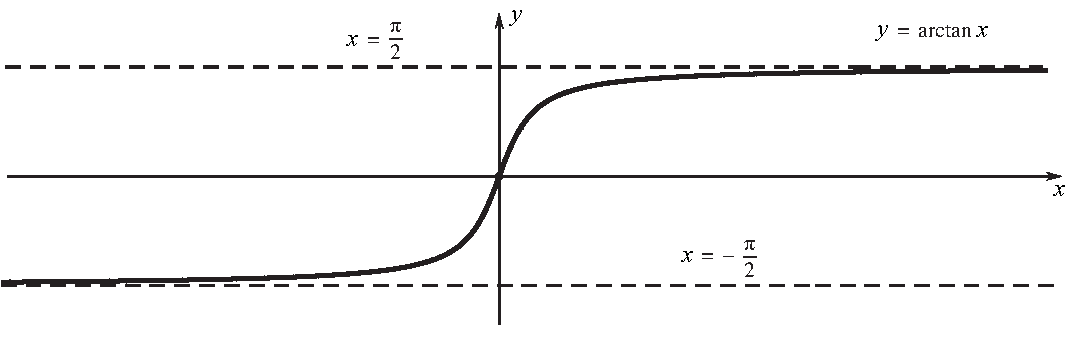
\includegraphics[width = 0.9\linewidth]{pic/C-F/arctan.pdf}
	\vspace*{-1em}
	\caption{$\arctan$函数的图像}
	\label{atan}
\end{figure}
$y = \arctan x$的函数图像如图 \ref{atan} 所示,其定义域为$(-\infty, + \infty)$,值域为$(-\pi/2, \pi/2)$.

\begin{figure}[!htb]
	\begin{minipage}{0.49\linewidth}
		\centering
		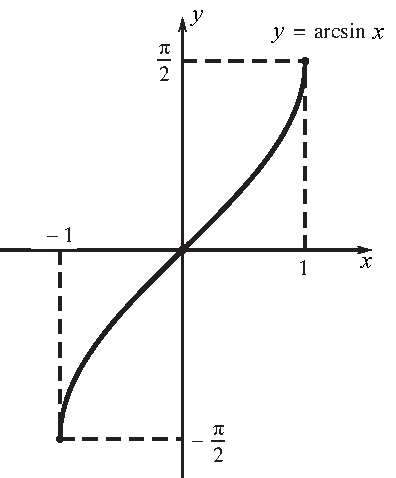
\includegraphics[width=0.89\linewidth]{pic/C-F/arcsin.pdf}
		\caption{$\arcsin$函数的图像}
		\label{asin}
	\end{minipage}
	\begin{minipage}{0.49\linewidth}
		\centering
		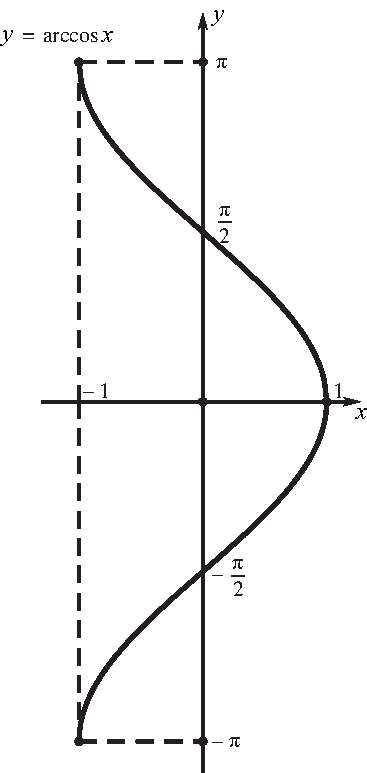
\includegraphics[width=0.51\linewidth]{pic/C-F/arccos.pdf}
		\caption{$\arccos$函数的图像}
		\label{acos}
	\end{minipage}
\end{figure}
$y = \arcsin x$的函数图像如图 \ref{asin} 所示,其定义域为$[-1, 1]$,值域为$[-\pi/2, \pi/2]$.

$y = \arccos x$的函数图像如图 \ref{acos} 所示,其定义域为$[-1, 1]$,值域为$[0, \pi)$.

\section{基本公式}
\vspace*{-2em}
\begin{align}
	\boxed{a^3 + b^3 = (a + b)(a^2 - ab + b^2)}\quad \quad  \\[0.5em]
	\boxed{a^3 - b^3 = (a - b)(a^2 + ab + b^2)}\quad \quad \\[0.5em]
	\boxed{(a + b)^2 = a^2 + 2ab + b^2 }\quad \quad \quad\,\,\\[0.5em]
	\boxed{(a - b)^2 = a^2 - 2ab + b^2 }\quad \quad \quad\,\,\\[0.5em]
	\boxed{(a-b)(a+b) = a^2 - b^2}\quad \quad \quad\,\,\\[0.5em]
	\boxed{x^n - 1 = (x - 1)(x^{n-1} + x^{n-2} + \cdots + x + 1)}
\end{align}
\proof 由等比数列求和公式:$x^{n-1} + x^{n-2} + \cdots + x + 1 = \dfrac{x^n - 1}{x -1}$,即$x^n - 1 = (x - 1)(x^{n-1} + x^{n-2} + \cdots + x + 1).$

\noindent 7. 当$n$为奇数时,$x^n + 1 = (x+1)(x^{n-1}- x^{n-2} + x^{n-3} - \cdots - x + 1)$;当$n$为偶数时,$x^n + 1$不能因式分解.

\warn[\quad 在我们做题化简应用公式的时候,我们通常会正用而不会或不记得要逆用。]

下面给出几个例子。\\[1em]
1. $\displaystyle \sqrt[3]{a} - \sqrt[3]{b} = \dfrac{\big(\sqrt[3]{a} \big)^3 - \big(\sqrt[3]{b} \big)^3}{\sqrt[3]{a^2} + \sqrt[3]{a}\cdot\sqrt[3]{b} + \sqrt[3]{b^2}} = \dfrac{a-b}{\sqrt[3]{a^2} + \sqrt[3]{ab} + \sqrt[3]{b^2}} \xrightarrow{\textstyle \,\, b = 1 \,\,} \sqrt[3]{a} - 1 = \dfrac{a-1}{\sqrt[3]{a^2} + \sqrt[3]{a} + 1}$\\[0.5em]
2. $\displaystyle \sqrt[3]{a} + \sqrt[3]{b} = \dfrac{\big(\sqrt[3]{a} \big)^3 + \big(\sqrt[3]{b} \big)^3}{\sqrt[3]{a^2} - \sqrt[3]{a}\cdot\sqrt[3]{b} + \sqrt[3]{b^2}} = \dfrac{a-b}{\sqrt[3]{a^2} -\sqrt[3]{ab} + \sqrt[3]{b^2}} \xrightarrow{\textstyle \,\, b = 1 \,\,} \sqrt[3]{a} + 1 = \dfrac{a+1}{\sqrt[3]{a^2} - \sqrt[3]{a} + 1}$\\[1em]
\par 对于极限$\displaystyle \dfrac{\sqrt[3]{a} - \sqrt[3]{b}}{a - b}$的形式往往是$\dfrac{0}{0}$型,通过上面的简化后,可以直接化简为
$$
\dfrac{\sqrt[3]{a} - \sqrt[3]{b}}{a - b} = \dfrac{1}{\sqrt[3]{a^2} + \sqrt[3]{ab} + \sqrt[3]{b^2}}
$$
这就很容易求得$\displaystyle \dfrac{\sqrt[3]{a} - \sqrt[3]{b}}{a - b}$的极限。

\begin{tcolorbox}[title=补充:平方差(和)为1的重要公式]
	\begin{align}
		\boxed{\sin^2 x + \cos^2 x = 1} \\[0.5em]
		\boxed{\sec^2 x - \tan^2 x = 1} \\[0.5em]
		\boxed{\ch x^2 - \sh^2 x = 1}\,\, \\[0.5em]
		\boxed{\csc^2 x - \cot^2 x = 1}
	\end{align}
	\qquad 对于求含有根号且根号内的两个数具备平方差(和)的关系时的积分,通常可以利用这几个公式进行三角换元,从而达到去根号(化繁为简)的效果。
\end{tcolorbox}
\vspace*{0.5em}

\section{有理化}
有理化分为分子有理化、分母有理化和分子分母同时有理化。

有理化在求极限中是十分常见的化简方法,因为它能将趋于0的减法根式变为不趋于0的加法根式并且可以构造约分。以下给出几个例子。

\examples 求下列极限:\\[1em]
1. $\displaystyle \lim\limits_{x \to 0} \dfrac{\sqrt{1+x} - \sqrt{1-x}}{x}$.\\[1em]
\solve 原式$\displaystyle = \lim \limits_{x \to 0} \dfrac{\big(\sqrt{1+x} - \sqrt{1-x} \big)\big(\sqrt{1+x} + \sqrt{1-x}\big)}{x\big( \sqrt{1+x} + \sqrt{1-x} \big)} = \lim \limits_{x \to 0} \dfrac{2x}{x\big( \sqrt{1+x} + \sqrt{1-x} \big)} = \lim \limits_{x \to 0} \dfrac{2}{\big( \sqrt{1+x} + \sqrt{1-x} \big)} = 1.$













